\documentclass{ceel}

% ===========================
%Coloque aqui pacotes adicionais, se necessário
\usepackage{hyperref}
\usepackage{verbatim}
\usepackage{array}
\usepackage{amsmath}
\usepackage{subcaption, float}
%%===========================

% Dados do trabalho
\title{Fundamentos Físico-químicos e Matemáticos de um Memristor}

%\author[1]{\underline{Lesly Viviane Montúfar Berrios}\thanks{leslymontufar@ufu.br}}
%\author[1]{Cibelly Cristina Rodrigues Couto\thanks{cibelly.cris@ufu.br}}
%\author[1]{Yasmin Delbany Cury\thanks{yasmin.cury@ufu.br}}
%\author[2]{Paulo Henrique Oliveira Rezende\thanks{paulohenrique.rezende@ufu.br}}

%\author[1]{\underline{Primeiro Autor Apresentador}\thanks{apresentador@ufu.br}}
%\author[1]{Nome do Segundo Autor\thanks{segundoautor@ufu.br}}
%\author[1]{Nome do Terceiro Autor \thanks{terceiroautor@ufu.br}}
%\author[2]{Nome do Autor Orientador\thanks{orientador@ufu.br}}
%
%
%\affil[1]{FEELT - Universidade Federal de Uberlândia}
%\affil[2]{FEELT - Professor Adjunto - Universidade Federal de Uberlândia}

\begin{document}

\inserirtitulo
\vspace{3cm}

\begin{multicols}{2}

\textbf{\emph{Resumo} - Um estudo sobre o comportamento do quarto elemento de circuito fundamental idealizado por Leon Chua em 1971 e implementado primeiramente pela equipe da \emph{HP Labs} liderada por R. Stanley Williams em 2008 é apresentado. Chamado de \emph{memristor}, o novo elemento de circuito passivo de duplo terminal relaciona as variáveis de carga $q(t)$ e fluxo $\varphi(t)$, e comporta-se como um resistor não-linear com memória. Sua propriedade peculiar advém da capacidade do material de manter seu último estado, e permite aplicações em diversos contextos, como em memórias ReRam e computação neuromórfica.} %% aplicacoes a completar
\vspace*{10pt}

\textbf{\emph{Palavras-Chave} - Aplicações, físico-químico, matemática, memristor.}


\begin{center}

%Insira aqui o Título do trabalho em inglês
\noindent\textbf{\large \uppercase{Physicochemical and Mathematical Foundations of a Memristor}}
\end{center}

\textbf{\emph{Abstract} - A study of the behavior of the fourth fundamental circuit element devised by Leon Chua in 1971 and first implemented by the \emph{HP Labs} team led by R. Stanley Williams in 2008 is presented. Called \emph {memristor}, the new two-terminal passive circuit element lists the variables of charge $q(t)$ and flux $\varphi(t)$, and behaves like a nonlinear resistor with memory. Its peculiar property comes from the material's ability to maintain its last state, and allows applications in various contexts, such as ReRam memories and neuromorphic computing.}
\vspace*{10pt}

\textbf{\emph{Keywords} - Applications, mathematics, memristor, physicochemical.}


\section{Introdução}
A teoria de circuitos elétricos, há 150 anos, abrangia basicamente três componentes passivos fundamentais: o capacitor (1745), o resistor (1827) e o indutor (1831). No entanto, em 1971, o professor phD da Universidade da Califórnia, Leon Chua, apresentou novas considerações a partir da análise das possíveis combinações entre as quatro variáveis fundamentais de circuitos: corrente elétrica $i$, tensão elétrica $v$, carga elétrica $q$ e fluxo magnético $\varphi$ – sendo as duas últimas descritas como integrais no tempo da corrente, $q(t)=\int_{-\infty}^t i(\tau)\, d\tau$, e da tensão, $\varphi(t)=\int_{-\infty}^t v(\tau)\, d\tau$, respectivamente.

Chua \cite{artigo} observou que o capacitor é definido pela relação entre carga $q(t)$ e tensão $v(t)$ via $qd=C dv$. Similarmente, o resistor pela relação entre corrente $i(t)$ e tensão $v(t)$ via $dv=R di$, e o indutor pela relação entre fluxo magnético $\varphi(t)$ e corrente $i(t)$ via $d\varphi(t)=L di$. Teria-se então que a combinação das quatro variáveis fundamentais de circuitos resultaria em somente três componentes fundamentais.
% passivos.
Desse modo, baseando-se no argumento da simetria, o estudioso postulou que haveria um elemento de circuito faltante, capaz de associar a carga $q(t)$ e o fluxo magnético $\varphi(t)$, o que o levou, em 1971, a publicar um artigo no qual idealiza o novo componente, definido pela relação $d\varphi=M dq$ e denominou-o \emph{memristor}, uma contração de \emph{memory resistor}. 

%, em português \emph{resistor com memória} 
Portanto, considerado como o quarto elemento fundamental dos circuitos eletrônicos, ao lado do capacitor, resistor e indutor, o \emph{memristor} destaca-se por apresentar uma propriedade peculiar, cuja explanação e abordagem teórica é tratada adiante. É definido, assim como um resistor, como um componente eletrônico passivo de duplo terminal, utilizado para limitar a corrente em um circuito e dissipar energia térmica, com o diferencial de que, para o \emph{memristor}, essa limitação, chamada de resistência ou impedância, altera-se conforme a quantidade de carga elétrica que flui em si e mantém o valor da última resistência obtida até a aplicação de nova carga.

Apesar da proposta teórica do \emph{memristor} ter sido apresentada por Chua em 1971, sua primeira implementação prática ocorreu apenas em 2008, nos \emph{Laboratórios da Hewllet-Packard} (\emph{HP}), graças à equipe liderada pelo físico-químico Dr. Richard Stanley Williams, que desenvolveu, em escala nanométrica, linhas de memristores com base no dióxido de titânio ($TiO_2$) \cite{nature}. A demora deve-se, principalmente, à dificuldade em encontrar materiais capazes de conferir a propriedade de reter memória ao dispositivo eletrônico e que satisfizessem a base teórica apresentada por Chua \cite{artigo}.
Dessa forma, o componente recentemente sintetizado contém a propriedade da não-volatilidade, que, aliada a possibilidade de ser trabalhado em escala nanométrica, o torna promissor em aplicações e garante sua contribuição na validação da Lei de Moore.

Pissardini \cite{memcomputacao} atenta para aplicações de \emph{memelementos} na elaboração de novas arquiteturas computacionais, que, corroborado pelos ideais da Arquitetura de Von Neumann, são capazes de realizar tarefas específicas. Essa abordagem tem sido conhecida como \emph{memcomputação}. Prezioso et al. \cite{rneurais} propõe também aplicações nas chamadas redes neurais, as quais são sistemas que se baseiam em princípios de Inteligência Artificial, podendo aprender e reconhecer padrões, e que podem ser aprimoradas com o uso da \emph{memresistência} devido ao caráter de não-volatilidade dos \emph{memristores}. Dong et al. \cite{chines}, em seu artigo acerca de circuitos lógicos, analisam a importância de memristores para otimizar seu funcionamento, devido à característica não linear que possuem.

Sob essa perspectiva, a temática deste artigo basear-se-á na descrição detalhada desse novo componente, nos âmbito físico, químico e matemático, com intuito de compreender como o mecanismo interno converge para as propriedades impostas,  por Chua \cite{artigo}, a um dispositivo \emph{memristor}. É de interesse ainda discutir acerca das aplicabilidades do dispositivo, para assim poder expor o impacto de sua descoberta na teoria de circuitos e importância para o crescimento tecnológico. %% eletronico com SPICE
%% se formos acrescentar mais alguma coisa como circuito LTSpice.
%% depende das aplicacoes

Na Seção \ref{estrutura} são apresentadas as características estruturais, físico-químicas, de um \emph{memristor}, com ênfase para o modelo da \emph{HP Labs}. Para, na Seção \ref{analise-matematica}, analisá-lo matematicamente e, assim, provar a natureza de suas propriedades e peculiaridades a partir do equacionamento e disposição de gráficos. Além disso, a Seção \ref{sim} apresenta simulações computacionais no ambiente \emph{MATLAB}
 e \emph{LTSPICE} que exemplificam suas características marcantes. Finalmente, na Seção \ref{aplicacoes}, é explicitada algumas de suas aplicações e recentes estudos.

%% precisa colocar imagem pequena para explicar que a propriedade do memristor deve-se basicamente à redistribuição das lacunas(+) devido à deficiencia em oxigenio.
%% de preferencia a msm imagem do R. Stanley Williams
\section{Características estruturais de um \emph{memristor}} \label{estrutura}
Dispositivos de resistência variável baseados em óxidos 
possuem vasta aplicabilidade, devido à capacidade de reter memória, pois
admitem características de alta velocidade, alta densidade e operação em baixa energia, 
assim como a não-volatilidade. Desse modo, materiais óxidos são ideiais para implementar o conceito de um dispositivo \emph{memristor}, sendo recentemente utilizados para esse fim os óxidos de titânio e tântalo ($TiO_x$, $TaO_x$) \cite{conceito}. %% Física do estado sólido

Para analisar o funcionamento de um memristor, é interessante compreender o dispositivo \emph{crossbarlatch}, estudado em 2006 pela
\emph{HP Labs}, que posteriormente passou a ser conhecido como o próprio \emph{memristor}. O crossbarlatch era uma espécie de sanduíche, possuindo partes externas constituídas por Platina ($Pt$), com espessura cerca de 3 nanômetros, e uma camada intermediária isolante subdividida em duas partes, uma formada de óxido de titânio ($TiO_2$), conhecida como parte pura ou não dopada, e outra pela mesma substância porém deficiente em oxigênio ($TiO_{2-x}$), conhecida como parte dopada \cite{construcao}.  Nesse sentido, o funcionamento molecular de um memristor é baseado no movimento de íons livres, no meio dielétrico (óxido), o que torna possível o comportamento memristivo, pois cria mudanças locais na condutividade a partir da modelagem de filamentos condutores entre os eletrodos.

Esses filamentos condutores são resultantes de um processo conhecido como \emph{eletroformação}, do inglês \emph{electroforming}, que consiste na aplicação de uma tensão elétrica suficientemente alta, ou seja um valor limite de tensão entre os dois eletrodos por um período de tempo suficiente para a formação de um canal condutivo local no meio isolante, o que significa o rompimento de sua rigidez dielétrica.
Ademais, esses valores limite de tensão e de tempo necessários para a formação do canal condutivo dependem dos materiais que constituem os dielétricos e os eletrodos, além da estrutura geométrica do dispositivo \cite{us}. 

\vspace{-0.25cm}
\begin{figure}[H]
\centering
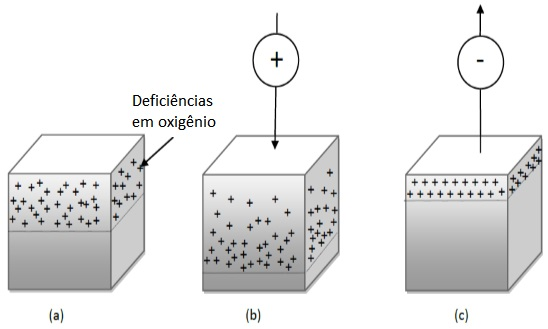
\includegraphics[width=\columnwidth]{modificado}
\caption{(a) Distribuição das vacâncias de oxigênio na camada intermediária de um memristor. (b) Aplicando-se tensão positiva os íons livres são repelidos. (c) Aplicando-se tensão negativa os íons livres são atraídos (Adaptado de \cite{study}).}\label{estrutura}
\end{figure}
\vspace{0.01cm}

Devido à flexibilidade de variação de valores de resistência, ao memristor podem ser atribuídos estados como “OFF”, quando a parte não-dopada é dominante portanto o estado é de alta resistência; “ON”, quando a parte dopada é dominante portanto há baixa resistência, e ainda estados intermediários. Assim, pode armazenar dados em multinível e não apenas na forma binária, como representado na Figura \ref{estrutura}(a). Observa-se também que as nanopartículas utilizadas na dopagem possuem carga $+2$ (vacâncias de oxigênio) e é representado um estado no qual há uma proporção igualitária entre parte dopada e não dopada em um memristor. 

Constata-se ainda que ao se aplicar uma tensão elétrica positiva 
no terminal dopado, a partir de um estado inicial qualquer como o da Figura \ref{estrutura}(a), as lacunas (vacâncias de oxigênio), que comportam-se como cargas positivas, migram para o lado oposto, ou seja, cargas negativas se deslocam para a parte dopada.
 Dessa forma, a espessura da camada intermediária não-dopada diminui, ao mesmo tempo que a espessura da camada dopada e de maior condutividade aumenta, o que resulta na diminuição do valor da resistência do dispositivo. Tal estado do memristor é conhecido como "ON", ou de baixa resistência, e é ilustrado na Figura \ref{estrutura}(b). 

Por outro lado, ao se aplicar uma tensão negativa no terminal dopado, as lacunas são atraídas, logo a espessura da camada intermediária não-dopada aumenta, ao mesmo tempo que a espessura da camada de maior condutividade diminui, causando um aumento no valor da resistência do memristor. Tal estado, ilustrado na Figura \ref{estrutura}(c), é conhecido como "OFF", ou de alta resistência. 

Assim, o princípio básico de funcionamento de um memristor consiste basicamente na redistribuição das lacunas sob a influência de uma tensão elétrica aplicada, que, quando cessada, tem-se ainda que camadas pura e dopada permanecem no último estado atingido. Dessa forma, são dispositivos capazes de memorizar o último valor de resistência alcançado, e esse processo é facilitado por ocorrer em escala nanométrica. %% por que? equacao 1/D^2

\section{Fundamentos Matemáticos}\label{analise-matematica}
O \emph{memristor}, a princípio, em 1971, foi definido por Chua \cite{artigo} como elemento de circuito de duplo-terminal caracterizado pela relação do tipo $g(\varphi, q)=0$. Diz-se que 
um memristor é controlado por carga se a relação entre fluxo e carga é expressa como uma função de carga elétrica $q$, e diz-se que é controlado por fluxo se é expressa em função do 
fluxo $\varphi$. Para um memristor controlado por carga tem-se a Equação (\ref{mem-charge}) e derivando-se ambos os termos consegue-se a Equação (\ref{derivate-q}).
\begin{equation}\label{mem-charge}
\varphi = f(q)
\end{equation}
\vspace{-0.2cm}
\begin{equation}\label{derivate-q}
\dfrac{d\varphi}{dt}=\dfrac{df(q)}{dq} \ \dfrac{dq}{dt}
\end{equation}
\vspace{0.05cm}

Sabendo-se ainda que $v(t)=\frac{d\varphi}{dt}$ e $i(t)=\frac{dq}{dt}$ descrevem, respectivamente, a tensão e a corrente elétrica no memristor, 
reescreve-se a Equação (\ref{derivate-q}) como na Equação (\ref{M}).

\begin{equation}\label{vMi}
v(t)=M(q)\ i(t)
\end{equation}
\noindent onde
\begin{equation} \label{M}
M(q) =\dfrac{df(q)}{dq}
\end{equation}

$M$ é chamada de \textit{memristência}, e é mensurada na mesma unidade que a resistência (\textit{Ohms} - $\Omega$). A memristência, definida pela Equação (\ref{M}), define uma relação linear entre tensão e corrente, enquanto a carga for constante. Logo, se $M$ é constante, o memristor comporta-se como um resistor.

Para um memristor controlado por fluxo tem-se a Equação (\ref{mem-flux}) e derivando-se ambos os termos, a Equação (\ref{derivate-phi}).
\begin{equation}\label{mem-flux}
q = f(\varphi)
\end{equation}
\vspace{-0.2cm}
\begin{equation}\label{derivate-phi}
\dfrac{dq}{dt}=\dfrac{df(\varphi)}{d\varphi} \ \dfrac{d\varphi}{dt}
\end{equation}
\vspace{0.04cm}

Reescrevendo a Equação (\ref{derivate-phi}) utilizando-se as definições de tensão e corrente tem-se a  Equação (\ref{iWv}).

\begin{equation}\label{iWv}
i(t)=W(\varphi)\ v(t)
\end{equation}
\noindent onde
\begin{equation} \label{W}
W(\varphi) =\dfrac{df(\varphi)}{d\varphi}
\end{equation}

\begin{figure}[H]
\centering
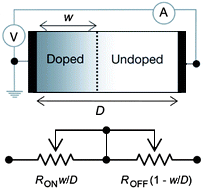
\includegraphics[width=0.7\columnwidth]{new-w}
\caption{Variáveis de estado de um memristor e representação de um memristor como uma associação em série de resistores \cite{image}.}\label{w}
\end{figure}

\vspace{0.2cm}
Nesse caso, $W$, da Equação (\ref{W}), é chamado de \textit{memductância} e tem mesma unidade da condutância (\textit{Siemens} - $S$).

Entretanto, em especial para o memristor controlado por por carga, as relações das Equações (\ref{vMi}) e (\ref{M}) não contemplam toda a interação física do componente, responsável por proporcionar a não-volatilidade ao dispositivo, o que levou Chua juntamente com seu então aluno de graduação Kang, em 1976, a fundamentar que o \emph{memristor} seria um componente passivo com \emph{estado}, ou seja, sua propriedade de memória define-se por uma ou mais \emph{variáveis de estado}.
Diante disso, a equipe \emph{HP Labs} pôde modelar matematicamente um memristor, a partir das equações para sistemas memristivos propostas por Chua e Kang \cite{1976} em (\ref{sm1}) e (\ref{sm2}).
\begin{equation}\label{sm1}
v=M(w, i)i
\end{equation}
\begin{equation}\label{sm2}
\dfrac{dw}{dt}=f(w, i)
\end{equation}
\vspace{0.00001cm}

Assim, a definição matemática rigorosa revela que, conforme a Equação (\ref{sm1}), a \emph{memristência} $M$ depende do estado do dispositivo descrito por $w$, que por sua vez, conforme a Equação (\ref{sm2}), varia com o tempo e referencia-se em uma função $f$ dependente do estado e da corrente através do memristor. Uma representação física de $w$ é ilustrada na Figura \ref{w}, a qual descreve o memristor como associação de duas resistências em série, $R_{ON}$ e $R_{OFF}$. Essa Figura também representa o primeiro modelo publicado pela equipe da \emph{HP Labs} \cite{nature}, no qual o transporte dos portadores de carga ocorre pelo \emph{Modelo de Deriva Linear}, que será explicado a seguir, mencionando os parâmetros padrões do projeto de sintetização do elemento, que serão utilizados inclusive nas simulações da Seção \ref{sim}.

Para o \emph{Modelo de Deriva Linear}, é primeiramente suposto um campo elétrico uniforme através do dispositivo, que resulta em uma relação linear entre a velocidade de deriva e o campo elétrico líquido. Assim, a memristência $M(w)$ define-se como na Equação (\ref{Mw}) e a relação geral para o movimento das nanopartículas positivas que é dada como $v_D=\mu\, E$ será descrita, nesse caso, pela Equação (\ref{vD}), sendo a mobilidade $\mu_D \sim 10^{-10} cm^2/V.s$, o comprimento do memristor utilizado $D\sim10nm$, $R_{ON}\sim 100\Omega$, $R_{OFF}\sim 16K\Omega$ e portanto $\Delta R = (R_{OFF} - R_{ON}) \approx R_{OFF}$ nos parâmetros típicos.
\columnbreak

\begin{equation}\label{Mw}
M(w)=\dfrac{w}{D}\, R_{ON}+\Big(1 - \dfrac{w}{D}\Big)\, R_{OFF}
\end{equation}

\begin{equation}\label{vD}
\dfrac{dw}{dt}=v_D=\dfrac{\mu_D R_{ON}}{D}i(t)
\end{equation}
\vspace{0.05cm}

Integrando-se a Equação (\ref{vD}) e depois dividindo seus termos por $D$ tem-se a Equação (\ref{wd}).
A partir dela, reescreve-se na Equação (\ref{qD}), pois tem-se que $Q_D=D^2/\mu_D R_{ON}$ é a carga necessária para mover a deriva de $w(t_0)$, onde $w\rightarrow 0$, para $w(t_D)$, onde $w\rightarrow D$.

\begin{equation}\label{wd}
\dfrac{w(t)}{D}=\dfrac{w_0}{D}+\dfrac{\mu_D R_{OFF}}{D^2}q(t)
\end{equation}

\begin{equation}\label{qD}
\dfrac{w(t)}{D}=\dfrac{w_0}{D}+\dfrac{q(t)}{Q_D}
\end{equation}
\vspace{0.04cm}

Ainda é possível estabelecer uma variável de estado $x(t)=w(t)/D$, e assim reescrever a Equação (\ref{qD}) como em (\ref{xt}) e a Equação (\ref{Mw}) como em (\ref{Mx}).

\begin{equation}\label{xt}
x(t)=x(t_0)+\dfrac{q(t)}{Q_D}
\end{equation}
\begin{equation}\label{Mx}
M(t)=R_{ON}\ x(t)+ R_{OFF}(1-x(t))
\end{equation}
\vspace{0.001cm}

Em $t_0$, define-se ainda $M_0$, dado pela Equação (\ref{t0}), em que $r=R_{OFF}/R_{ON}$. Logo, substituindo (\ref{xt}) em (\ref{Mx}) tem-se (\ref{M:M0}) ou (\ref{M:ROFF}), já que para $R_{OFF}\gg R_{ON}$, tem-se que $M_0\approx R_{OFF}$.
\vspace{0.05cm}

\begin{equation}\label{t0}
M_0  =R_{ON}\big( x(t_0)+ r\ (1-x(t_0))\big)
\end{equation}
\begin{equation}\label{M:M0}% essa direto
M(q)=M_0-\Delta R\, \bigg(\dfrac{q(t)}{Q_D}\bigg)
\end{equation}

\begin{equation}\label{M:ROFF}% exclui essa talvez
M(q)=R_{OFF}\bigg( 1-\dfrac{q(t)}{Q_D}\bigg)
\end{equation}
\vspace{0.04cm}

Substituindo (\ref{M:M0}) em (\ref{vMi}) tem-se que a tensão $v(t)$ é dada pela Equação (\ref{dt}) e integrando no tempo, sabendo que $\varphi(t)=\int_{-\infty}^t v(\tau)\, d\tau$ e $M(q)=d\varphi/dq$,  consegue-se definir $q(t)$ como na Equação (\ref{qt}), a partir das raízes da equação quadrática resultante.
%
\begin{equation}\label{dt}
v(t)=\Big(M_0-\Delta \, R\Big(\dfrac{q(t)}{Q_D}\Big)\Big)\dfrac{dq}{dt} = \dfrac{d}{dt} \Big(M_0\, q-\dfrac{\Delta R\, q^2(t)}{2 Q_D}\Big)
\end{equation}

\begin{equation}\label{qt}
q(t)=\dfrac{Q_D\ M_0}{\Delta R}\Bigg(1\pm\sqrt{1-\dfrac{2\, \Delta R}{Q_D\ M^2_0}\varphi(t)}\Bigg)
\end{equation} 
\vspace{0.04cm}

Utilizando-se novamente que $\Delta R \approx M_0 \approx R_{OFF}$, a Equação (\ref{qt}) resulta na (\ref{q}). 
\vspace{0.05cm}

\begin{equation}\label{q}
q(t)=Q_D\Bigg(1-\sqrt{1-\dfrac{2}{Q_D\ R_{OFF}}\varphi(t)}\Bigg)
\end{equation} 
\vspace{0.05cm}

Tem-se ainda que (\ref{q}) em (\ref{xt}) resulta no estado interno do memristor definido como em (\ref{interno}). Constata-se ainda que (\ref{q}) em (\ref{M:ROFF}) resulta em (\ref{nano}).
\begin{equation}\label{interno}
x(t)=1-\sqrt{1-\dfrac{2\, \mu_D}{r\; D^2}\varphi(t)}
\end{equation} 
\begin{equation}\label{nano}
M(q)=R_{OFF}\Bigg(\sqrt{1-\dfrac{2\, \mu_D}{r\; D^2}\varphi(t) }\Bigg)
\end{equation}
\vspace{0.05cm}

Portanto a corrente $i(t)$ é descrita como na Equação (\ref{i}).
\begin{equation}\label{i}
i(t)=\dfrac{v(t)}{R_{OFF}\Bigg(\sqrt{1-\dfrac{2\, \mu_D}{r\; D^2}\varphi(t) }\Bigg)}
\end{equation} 

Verifica-se que a Equação (\ref{nano}) mostra a relação inverso-quadrado entre a memristência $M$ e a espessura do $TiO_2$, $D$. Assim, para menores valores de $D$, a memória apresenta características melhoradas. Portanto, a memristência torna-se mais importante para a compreensão do porquê das dimensões dos dispositivos eletrônicos estarem diminuido para a escala nanométrica.

\section{Simulações} \label{sim}
O memristor possui características marcantes que serão interpretadas graficamente via programação \emph{MATLAB} a partir das Equações (\ref{q}), (\ref{interno}) e (\ref{i}). Considere um memristor com mobilidade $\mu_D \sim 10^{-10\,} cm^2/V.s$, comprimento $D\sim10nm$, e resistências do estado \textit{ON} e \textit{OFF}, $R_{ON}\sim 100\Omega$ e $R_{OFF}\sim 16K\Omega$, respectivamente. Como $\varphi(t)=\int_{-\infty}^t v(\tau)\, d\tau$, tem-se que para uma tensão senoidal do tipo $v(t)=v_0\cdot sin(\omega t)$, o fluxo é descrito pela Equação (\ref{flux}), em que $v_0$ é a amplitude da tensão de entrada e $\omega$ a frequência em \textit{rad/s}.

\begin{equation}\label{flux}
\varphi(t) = \dfrac{v_0\, (1-cos(\omega t))}{\omega}
\end{equation}

Sabendo-se que a potência em elementos passivos $p(t)$ deve ser sempre positiva para qualquer tempo $t$ e que a potência instantânea dissipada por um memristor define-se pela Equação (\ref{pot}), é preciso que a memristência $M(q)$ seja não-negativa, isto é $M(q)\geq 0$. Graficamente na Figura \ref{flux-charge}, tem-se $M(q)$ dada como a inclinação da curva $\varphi$-$q$, que será, portanto, sempre monótona crescente \cite{artigo}.
\begin{equation}\label{pot}
p(t) = v(t)i(t)=M(q(t))[i(t)]^2
\end{equation}

Na Figura \ref{vt:xt} comtempla-se como a variável de estado $x(t)\in[0,1]$ varia conforme a tensão aplicada $v(t)$ resultante do efeito da histerese no material. % comentar ...
%
Já na Figura \ref{pinched} é representada uma importante característica do memristor. O gráfico em laço ou o \emph{pinched hysteresis loop}, como denominado por Chua, corresponde à curva  $v$-$i$ de um memristor e possui a forma de uma Curva de Lissajous centrada na origem. A configuração deve-se ao fenônemo da histerese, que permite conservar a o útimo valor de memristência mesmo sem o potencial originalmente aplicado.

No simulador \emph{SPICE}, o circuito da Figura \ref{spice:project} permite obter a curva $v$-$i$ da Figura \ref{spice:pinched}, do que surge o seguinte teorema fundamental que "todo dispositivo de duplo terminal que exibe um \emph{pinched hysteresis loop} no plano tensão-corrente quando conduzido por um sinal DC e/ou senoidal de qualquer frequência é um sistema memristivo"  \cite{you}. Dessa forma, desde que o sistema continue no regime dos memristores, qualquer polarização simétrica de tensão de corrente alternada resulta em uma histerese de laço duplo, que colapsa em uma linha reta para altas frequências, conforme a Figura \ref{pinched}. O fenônemo também é vísivel em \ref{spice:vt-it}, a tendência do material de manter suas propriedades proporciona certa deformação da curva da corrente $i(t)$ no tempo, comparada com a curva da tensão de entrada $v(t)$.
\begin{figure*}[ht]
%\centering
\begin{subfigure}{0.33\textwidth}
%\centering
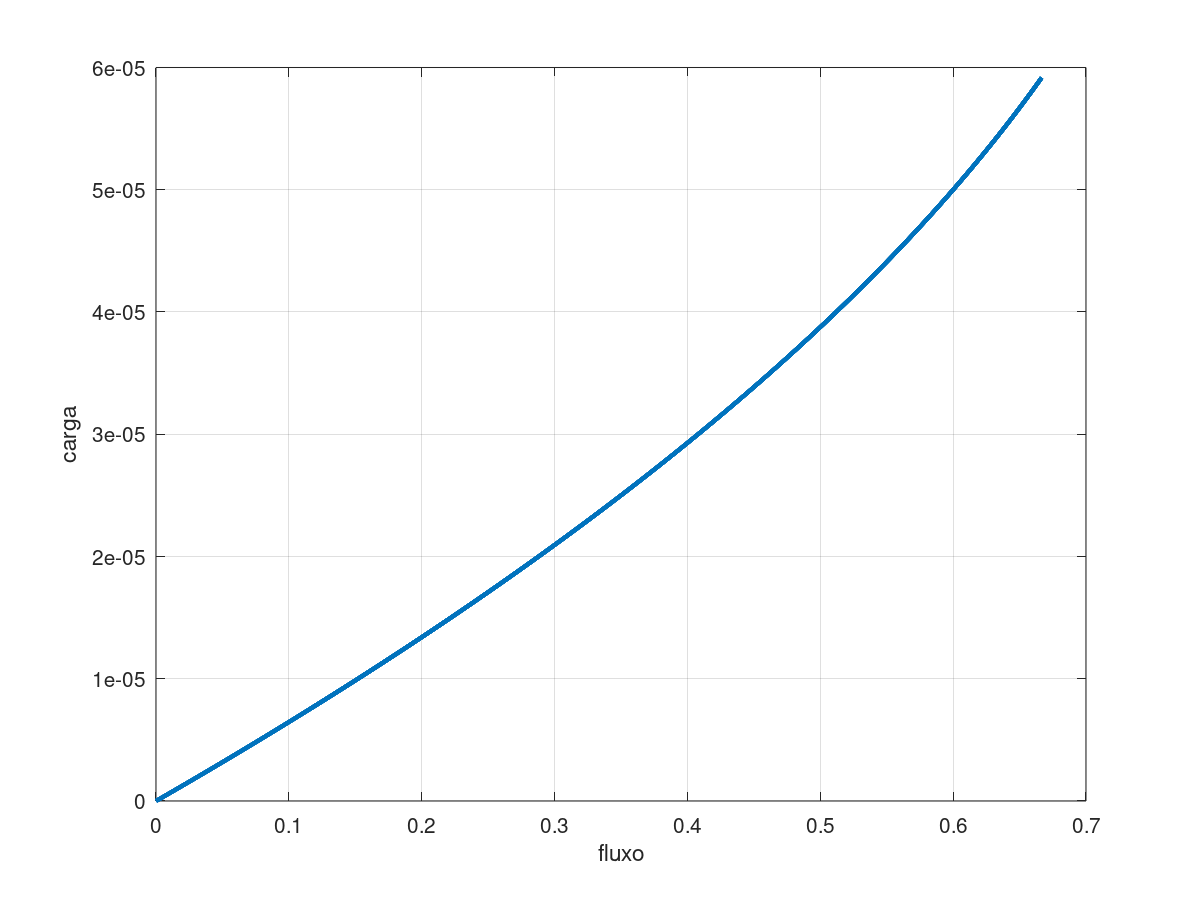
\includegraphics[width=\columnwidth]{flux-charge}
\caption{} \label{flux-charge}
\end{subfigure}
\hfill
\begin{subfigure}{0.33\textwidth}
%\centering
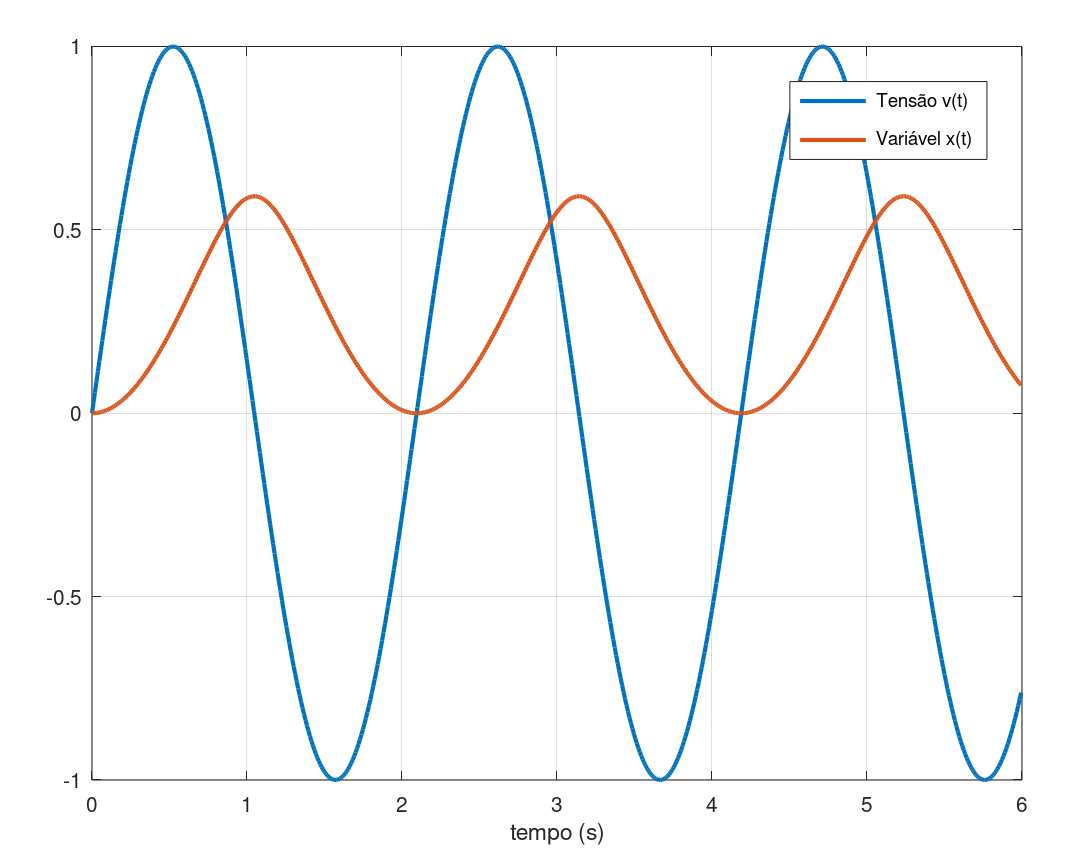
\includegraphics[width=\columnwidth]{vt-xt}
\caption{} \label{vt:xt}
\end{subfigure}
\hfill
\begin{subfigure}{0.33\textwidth}
\centering
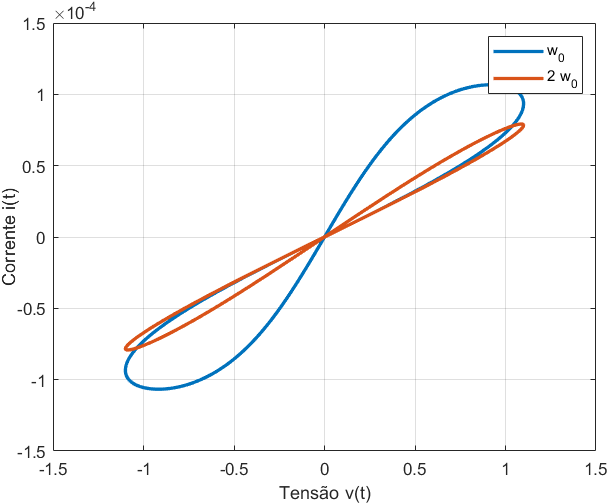
\includegraphics[width=\columnwidth]{ww0}
\caption{} \label{pinched}
\end{subfigure}

\vspace{0.2cm}
\begin{subfigure}{0.32\textwidth}
\centering
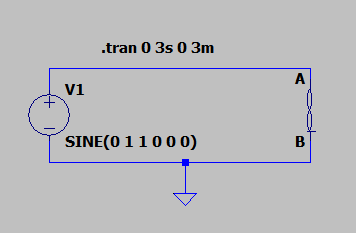
\includegraphics[width=\columnwidth]{ltspice}
\caption{} \label{spice:project}
\end{subfigure}
\hfill
\begin{subfigure}{0.32\textwidth}
\centering
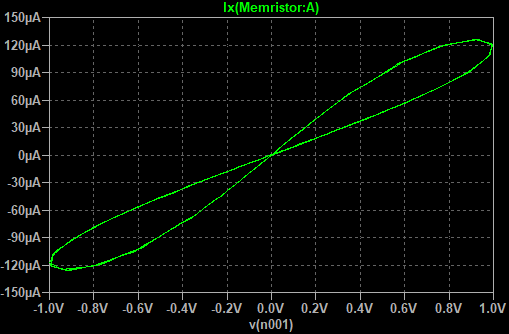
\includegraphics[width=\columnwidth]{pinched}
\caption{} \label{spice:pinched}
\end{subfigure}
\hfill
\begin{subfigure}{0.32\textwidth}
\centering
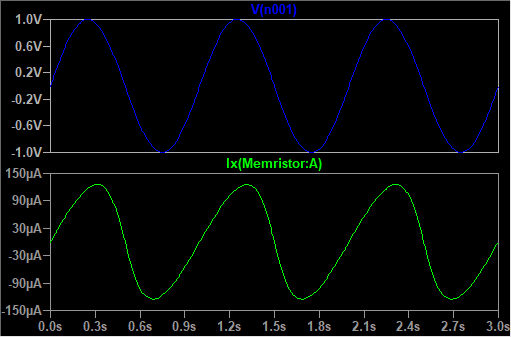
\includegraphics[width=\columnwidth]{vt-it}
\caption{} \label{spice:vt-it}
\end{subfigure}

\caption{No ambiente \textit{MATLAB} foram gerados os gráficos de (a)-(c), enquanto que (d)-(f) são obtidos pelo ambiente \textit{LTSPICE}. (a) Curva $\varphi$-$q$ de um memristor. (b) Relação entre a tensão de entrada $v(t)$ e a variável de estado $x(t)$ no tempo. (c) Curva $v$-$i$ de um memristor, chamado de \emph{pinched hysteresis loop} por Chua. (d) Esquema de simulação \textit{LTSPICE}. (e) \emph{Pinched hysteresis loop} de (d). (f) Curvas de tensão de entrada $v(t)$ e $i(t)$ no tempo, no qual observa-se o efeito da histerese sobre a corrente no dispositivo.}\label{simulacao}
\end{figure*}
%% Lisajous Figures


\section{Aplicações}\label{aplicacoes}
\subsection{Memórias ReRam}
A Memória Resistiva de Acesso Randômico (ReRAM) mantém os dados na falta de energia, essa propriedade deve-se especialmente pela presença do memristor em seus chips, que altera sua resistência de acordo com a passagem da corrente elétrica em resposta a variações na sua tensão de alimentação.
Essa tecnologia assemelha ao uso de transistores nas memórias Flash, com a diferença de as células de memória ReRAM serem muito menores, consumirem menos energia elétrica e armazenarem os dados como resistência, ao invés de armazenar como carga elétrica.

O ReRAM, portanto, tem o potencial de ser extremamente denso, de baixa potência, com alta resistência, tornando-se uma tecnologia atraente para armazenamento secundário e níveis de memória de classe de armazenamento \cite{prog}. Segundo a HP, dispositivos contendo memristores oferecem cerca de 20GB por centímetro quadrado, o dobro da capacidade projetada para as memórias flash.
Dispositivos memresistivos podem mudar o paradigma padrão da computação ao permitir que cálculos sejam executados nos chips onde a informação está armazenada \cite{hp}. Além disso, essa tecnologia é útil em todo tipo de dispositivo eletrônico.

\subsection{Circuitos híbridos CMOS} %  logic, hybrid circuits with CMOS, and neuromorphic computing.
Os circuitos híbridos combinam flexibilidade, confiabilidade e alta funcionalidade do subsistema CMOS com alta densidade de filme fino. Dispositivos memristivos não são componentes ativos, isto é, não podem fornecer energia para o circuito. A solução para esse problema é complementar matrizes de crossbar de dispositivos memristivos com um substrato CMOS convencional que fornece sinalização de restauração e ganho \cite{um}\cite{dois}.

%A Figura \ref{cibelly} mostra um exemplo de tais circuitos, c
Conhecido como CMOL (Dispositivos  híbridos Cmos + MOLecular). A combinação de circuitos CMOS e memristores não só tem um potencial para prolongar a Lei de Moore para memórias digitais e circuitos lógicos booleanos reconfiguráveis, mas também podem reviver o campo da computação neuromórfica artificial.
 
A tecnologia de circuitos híbridos é ajustada para fornecer maior conectividade entre pequenas células de circuito CMOS (escala de 100 portas) através de ligações “memristor de nanofios-nanofios”. Isso permite construir redes neuromórficas de larga escala com bom custo-benefício. Dispositivos memristivos são a base para as "sinapses", ou seja, comunicação entre as células. Consequentemente, redes neurais baseadas em CMOL podem ser eficientes, principalmente, no reconhecimento e classificação de padrões \cite{oito}.

\section{CONCLUSÕES}
O \emph{memristor}, idealizado por Chua em 1971, é considerado o quarto elemento fundamental de circuito, ao lado do capacitor, resistor e indutor. Implementado apenas em 2008 pela \emph{HP Labs}, o novo componente tem o diferencial de possuir a propriedade da não-volatilidade, que permite aplicá-lo em distintos contextos, podendo revolucionar desenhos de circuitos digitais e sistemas computacionais, além de representar um caminho inédito e possível à inteligência artificial. Diante de sua relevância para a teoria de circuitos, neste artigo são apresentados os fundamentos básicos de um \emph{memristor}, via ambientes \emph{MATLAB} e \emph{LTSPICE}, priorizando a explanação das características físico-químicas e matemáticas do primeiro sintetizado, ou seja, do modelo elaborado pela \emph{HP Labs}. 
Desse modo, seu estudo é de extrema importância para o desenvolvimento de áreas como nanotecnologia, microeletrônica, computação e inteligência artificial, e, embora pouco conhecido, o memristor já é aproveitado, por exemplo, nas memórias ReRam, tornando-as mais eficientes, por armazenar dados no próprio \emph{hardware}, e nos circuitos híbridos, por aprimorar a comunicação entre pequenas células de circuitos neuromórficos. 
%==================================
% REFERÊNCIAS
%==================================
\begin{thebibliography}{9}

%% INTRODUCAO
\bibitem{artigo}	
    L. Chua,
    “Memristor - the missing circuit element”, 
    in \emph{IEEE Transactions on circuit theory}, VOL. CT-18, NO. 5, Setembro 1971.

\bibitem{nature}	
     D.B. Strukov, G.S. Snider, D.R. Stewart,  R.S Williams, 
"The missing memristor found", 
\emph{Nature}, 2008, 1 May 2008, vol. 453, pp. 80-83.

\bibitem{memcomputacao}
    R. S. Pissardini,
    “Memcomputação: Características e Aplicações em Computação Paralela”, 
    Escola Politécnica da Universidade de São Paulo, Departamento de Engenharia de Transportes, Laboratório de Topografia e Geodesia.
% Disponível em: \url{https://www.ime.usp.br/~gold/cursos/2015/MAC5742/reports/MemComputacao.pdf}. Acesso em: jun. 2019.
 
 \bibitem{rneurais}	
   M. Prezioso, F. Merrikh-Bayat, B. D. Hoskins, G. C. Adam, K. K. Likharev, D. B. Strukov, "Training and operation of anintegrated neuromorphic
network based on metal-oxide memristors", 
Department of Electrical and Computer Engineering, University of California, California 93106, USA. 
Department of Physics and Astronomy, Stony Brook University, New York 11794, USA. 
%Disponível em: https://www.ece.ucsb.edu/~strukov/papers/2015/Nature2015.pdf. Acesso em ago. 2019.

\bibitem{chines}
    Z. Dong, D. Qi, Y. He, Z. Xu, X. Hu, S. Duan, "Easily Cascaded Memristor-CMOS Hybrid Circuit
for High-Efficiency Boolean Logic Implementation", School of Computer and Information Science,
College of Electronics and Information Engineering,
Southwest University, Chongqing 400715, P. R. China.
% Disponível em:\url{https://www.researchgate.net/publication/329039458\_Easily\_Cascaded\_Memristor-CMOS\_Hybrid\_Circuit\_for\_High-Efficiency\_Boolean\_Logic\_Implementation}. Acesso em ago. 2019.

%% FUNCIONAMENTO ESTRUTURAL
\bibitem{conceito}	
    J. P. Strachan, A. C. Torrezan, F. Miao, M. D. Pickett, J. J. Yang; W. Yi, G. M. Ribeiro, R. S. Williams,
 “State Dynamics and Modeling of
Tantalum Oxide Memristors”. 
Disponível em: 
\url{https://ieeexplore.ieee.org/stamp/stamp.jsp?arnumber=6542012}. Acesso em ago. 2019.
%https://ieeexplore.ieee.org/stamp/stamp.jsp?arnumber=6542012. Acesso em ago. 2019. 

\bibitem{construcao}	
   F.S.Barachati, "Estudo e Preparação de Memoristores para sua Aplicação em Dispositivos Eletrônicos", Escola de Engenharia de São Carlos, da Universidade de São Paulo. 
% Disponível em: \url{http://www.tcc.sc.usp.br/tce/disponiveis/18/180450/tce-26032012-090929/publico/Barachati_Fabio_Souza.pdf}.  Acesso em ago. 2019.   

\bibitem{us}	
    United States Patent; Patent No: US 9035272 B2.
    “Nanoparticle-Based Memristor Structure”. 
    Disponível em: 
\url{https://patentimages.storage.googleapis.com/0e/70/e0/6b8926f49e7cd8/US9035272.pdf}. Acesso em ago. 2019.
%    https://patentimages.storage.googleapis.com/0e/70/e0/6b8926f49e7cd8/US9035272.pdf. Acesso em ago. 2019.

%% MATEMATICA
\bibitem{study}	
    K. Kekur,
    “A Study of the Memristor, the Fourth Circuit Element”, 
   B.E., Visvesvaraya Technological University, 2007.

\bibitem{image}	
Y. Yang, W. Lu,
"Nanoscale resistive switching devices: mechanisms and modeling",
in \emph{Nanoscale},
2013, Vol. 5, 10076-10092, \emph{The Royal Society of Chemistry}, 10.1039/C3NR03472K. 
%Disponível em: \url{http://dx.doi.org/10.1039/C3NR03472K}. Acesso em ago. 2019.

\bibitem{1976}	
    L. Chua, S. M. Kang,
    “Memristive devices and systems”, 
    in \emph{Proceedings IEEE}, 1976, vol. CT-18, no. 5, pp. 507-519.

\begin{comment}
\bibitem{elusive} % indescritivel
    Y. N. Joglekar, S. J. Wolf, "The elusive memristor: properties of basic electrical circuits", Department of Physics, Indiana University Purdue, 2009.
\end{comment}

\bibitem{you} % indescritivel
    L. Chua,
    "Memristor and Memristive Systems Symposium",  UC Berkeley Events, 2008.
    Disponível em: 
%\url{https://www.youtube.com/watch?v=QFdDPzcZwbs}. Acesso em ago. 2019.
https://www.youtube.com/watch?v=QFdDPzcZwbs. Acesso em ago. 2019.

%% APLICACOES

%% MEMORIAS RERAM
\bibitem{prog}
    M. Ramadan, N. Wainstein, R. Ginosar, S. Kvatinsky, 
   "Adaptive programming in multi-level cell ReRAM", Microelectronics Journal, Volume 90, 2019. %% MULTI-LEVEL CELL == MLC ?!
    %% bem recente :)
    
\bibitem{hp}
     A. Martins, 
	"ReRam – A próxima geração de Memórias e CPU’s", 2010. 
	Disponível em: 
%\url{https://brainstormdeti.wordpress.com/2010/09/15/reram-\%E2\%80\%93-a-proxima-geracao-de-memorias-e-cpu\%E2\%80\%99s/}. Acesso em ago.2019
https://brainstormdeti.wordpress.com/2010/09/15/reram-\%E2\%80\%93-a-proxima-geracao-de-memorias-e-cpu\%E2\%80\%99s/. Acesso em ago.2019

%% CIRCUITOS LOGICOS
\bibitem{um}
K.K. Likharev, “Electronics below 10 nm”, in \emph{Nano and Giga Challenges in Microelectronics}, J. Greer et al., Eds., Amsterdam: Elsevier, pp. 27-68, 2003.

\bibitem {dois}
D. J. Frank, D. J. Frank, R. H. Dennard, E. Nowak, P. M. Solomon, Y. Taur, and H. S. P. Wong, 
“ Device scaling limits of Si MOSFETs and their application dependencies”, 
\emph{Proceedings IEEE}, vol. 89(3), pp. 259–288, 2001.

\bibitem {oito}
K.K. Likharev, A. Mayr, I. Muckra, and Ö. Türel, 
“CrossNets: HighPerformance Neuromorphic Architectures for CMOL Circuits”, Ann. New York Acad. Sci., vol 1006, pp. 146-163, 2009.

\end{thebibliography}

\end{multicols}
\end{document}
